\documentclass{beamer}

\usefonttheme{professionalfonts} % using non standard fonts for beamer
\usefonttheme{serif} % default family is serif

\usepackage{hyperref}
%\usepackage{minted}
\usepackage{animate}
\usepackage{graphicx}
\def\Put(#1,#2)#3{\leavevmode\makebox(0,0){\put(#1,#2){#3}}}
\usepackage{colortbl}
\usepackage{tikz}
\usepackage{amssymb}
\usepackage{enumerate}
\usepackage{arydshln}
\usepackage{algorithm}
\usepackage{algpseudocode}

\colorlet{lightred}{red!25}
\colorlet{lightgreen}{green!25}
\beamertemplatenavigationsymbolsempty

\newcommand\blfootnote[1]{%
  \begingroup
  \renewcommand\thefootnote{}\footnote{#1}%
  \addtocounter{footnote}{-1}%
  \endgroup
}

\makeatletter

%% Textclass specific LaTeX commands.
\newcommand\makebeamertitle{\frame{\maketitle}}%
\AtBeginDocument{%
  \let\origtableofcontents=\tableofcontents
  \def\tableofcontents{\@ifnextchar[{\origtableofcontents}{\gobbletableofcontents}}
  \def\gobbletableofcontents#1{\origtableofcontents}
}
%% User specified LaTeX commands.
\usetheme{Malmoe}
\useoutertheme{infolines}
\addtobeamertemplate{headline}{}{\vskip2pt}
\setbeamercovered{transparent}

\makeatother

%%%%%%%%%%%%%%%%%%%%%%%%%%%%%%%%%%%%%%
%% Main document
%%%%%%%%%%%%%%%%%%%%%%%%%%%%%%%%%%%%%%
\begin{document}
\title[PFLOCK report]{PFLOCK Report}
\author[AC]{Andres Calderon}
\institute[Fall'20]{University of California, Riverside}
\makebeamertitle
\newif\iflattersubsect

\AtBeginSection[] {
    \begin{frame}<beamer>
    \frametitle{Outline} 
    \tableofcontents[currentsection]  
    \end{frame}
    \lattersubsectfalse
}

\AtBeginSubsection[] {
    \begin{frame}<beamer>
    \frametitle{Outline} 
    \tableofcontents[currentsubsection]  
    \end{frame}
}

\begin{frame}{Testing new approach}
    \begin{itemize}
        \item Compare with BFE.  Working with a 10K points dataset (BFE outputs errors with the current dense dataset [Killed]).
        \item Using different  values for epsilon from 2 to 10m.
        \item Results are the same.  Dealing with just minor issues about precision.
        \item Could we do better to handle maximal cliques when MBC is greater than $\epsilon$?
        \item What is the shape of those cliques?
    \end{itemize}
\end{frame}

\begin{frame}{The `widest' shape of a clique}
    \centering
    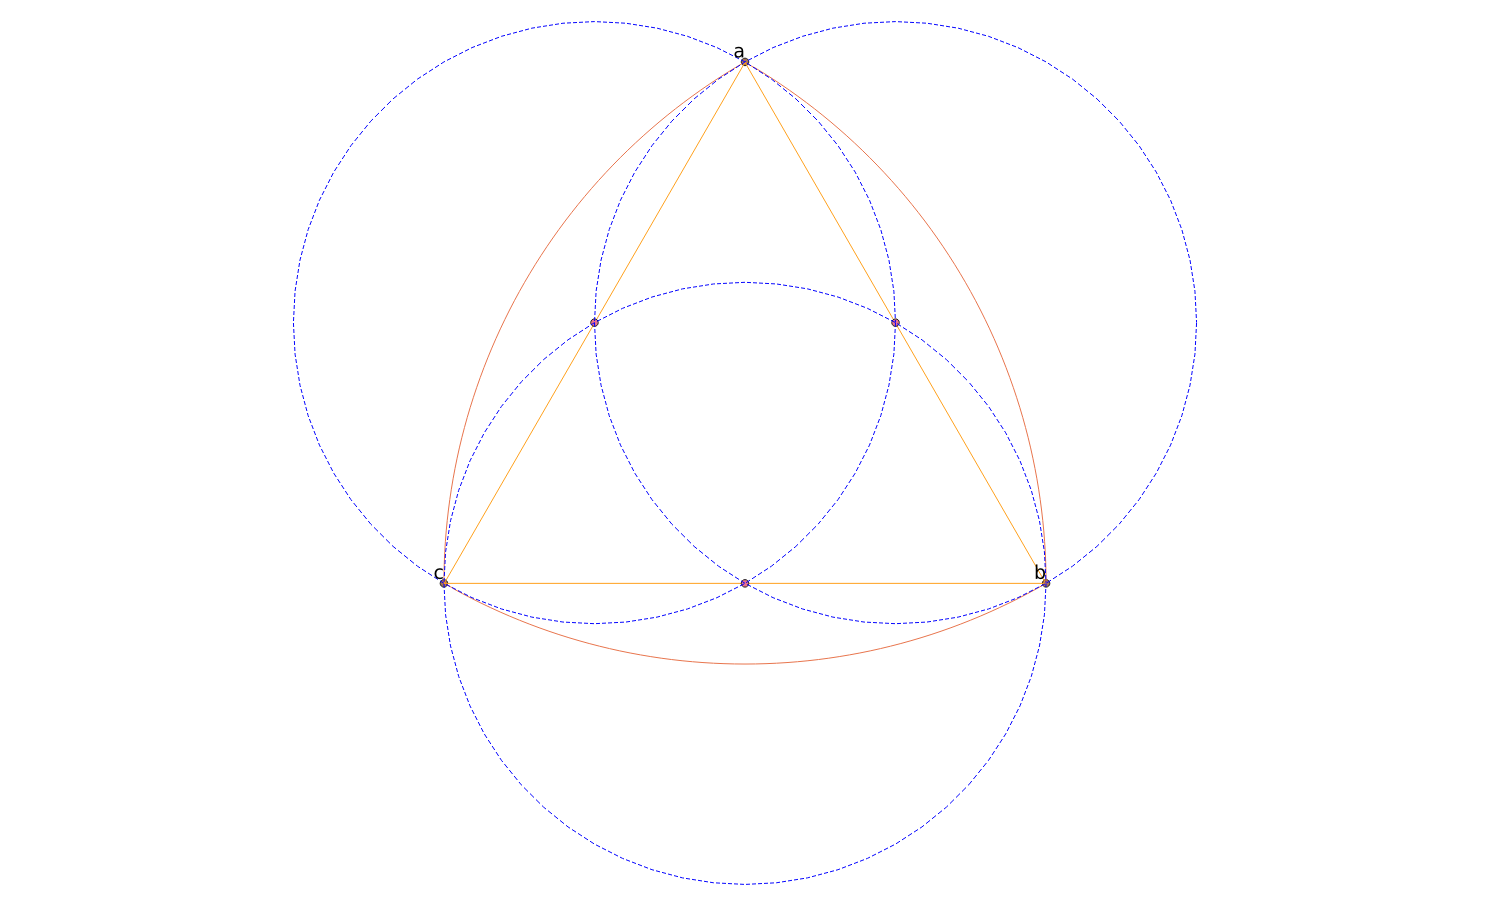
\includegraphics[width=0.85\textwidth]{figures/shape}
    \begin{itemize}
     \item The challenge will be the position and orientation of the shape...
    \end{itemize}

\end{frame}

\begin{frame}{A first attempt...}{Given a maximal clique}
    \centering
    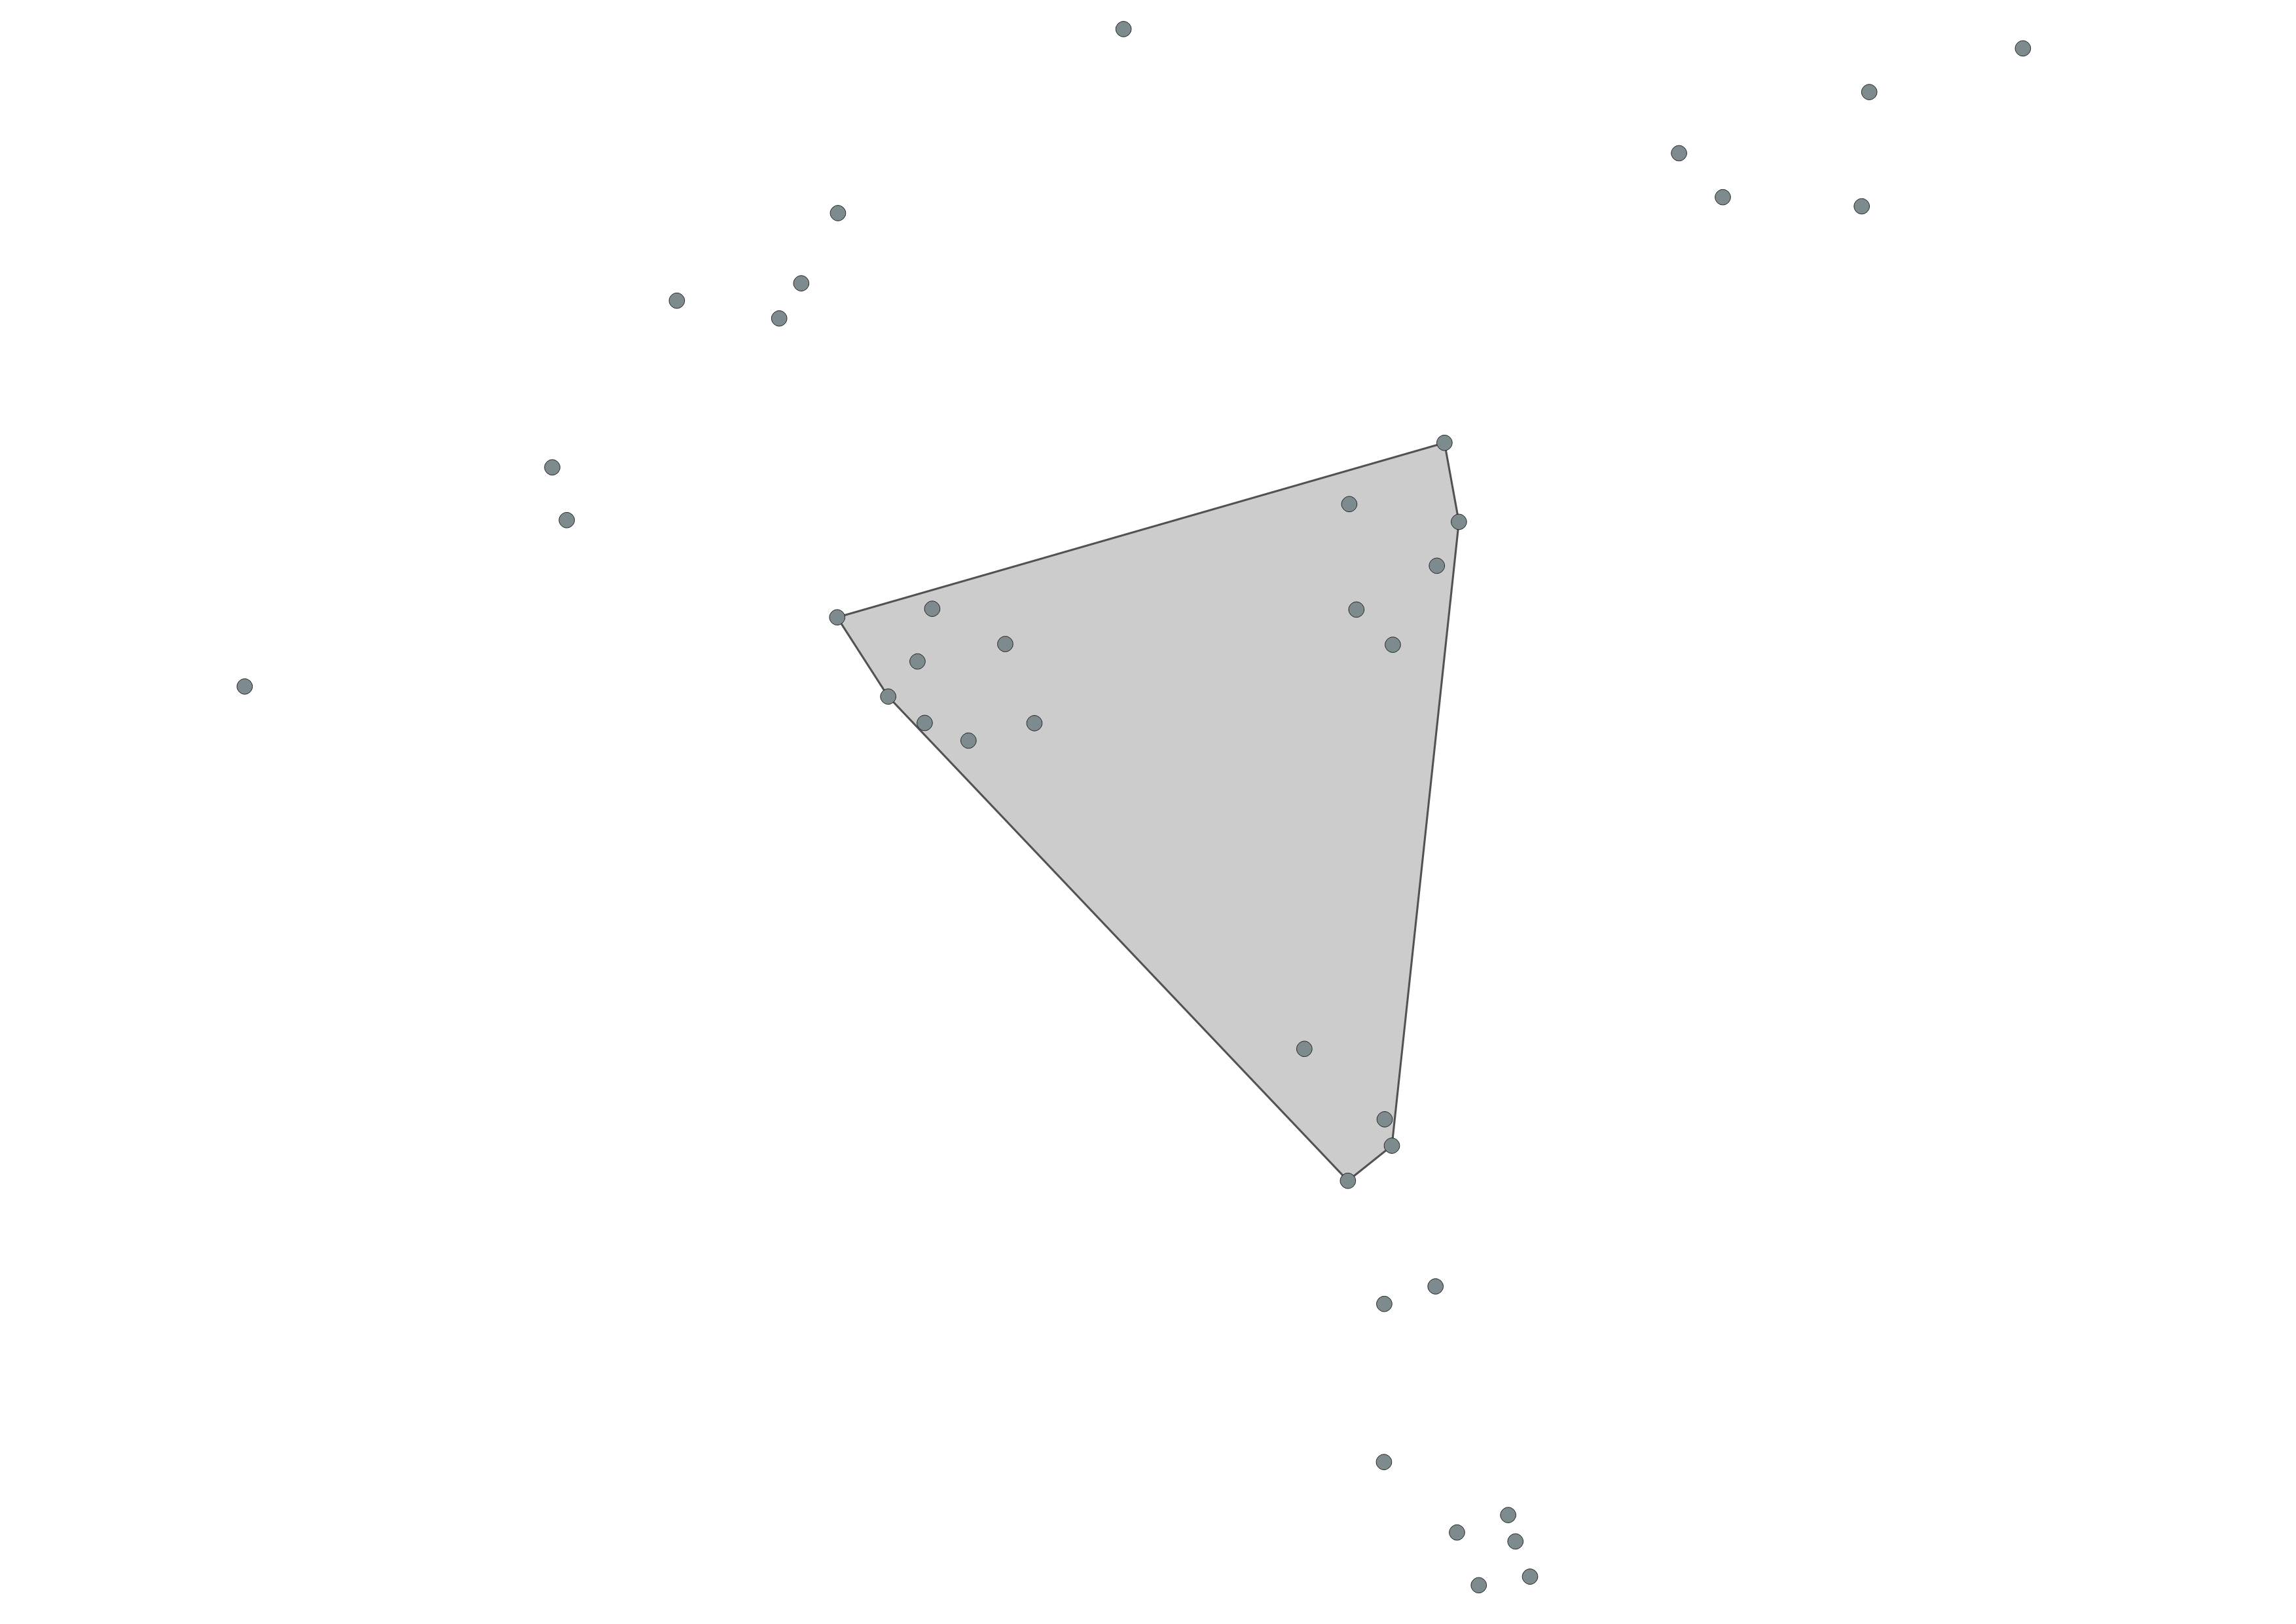
\includegraphics[width=0.85\textwidth]{figures/clique_69}
\end{frame}
\begin{frame}{A first attempt...}{Find the longest segment}
    \centering
    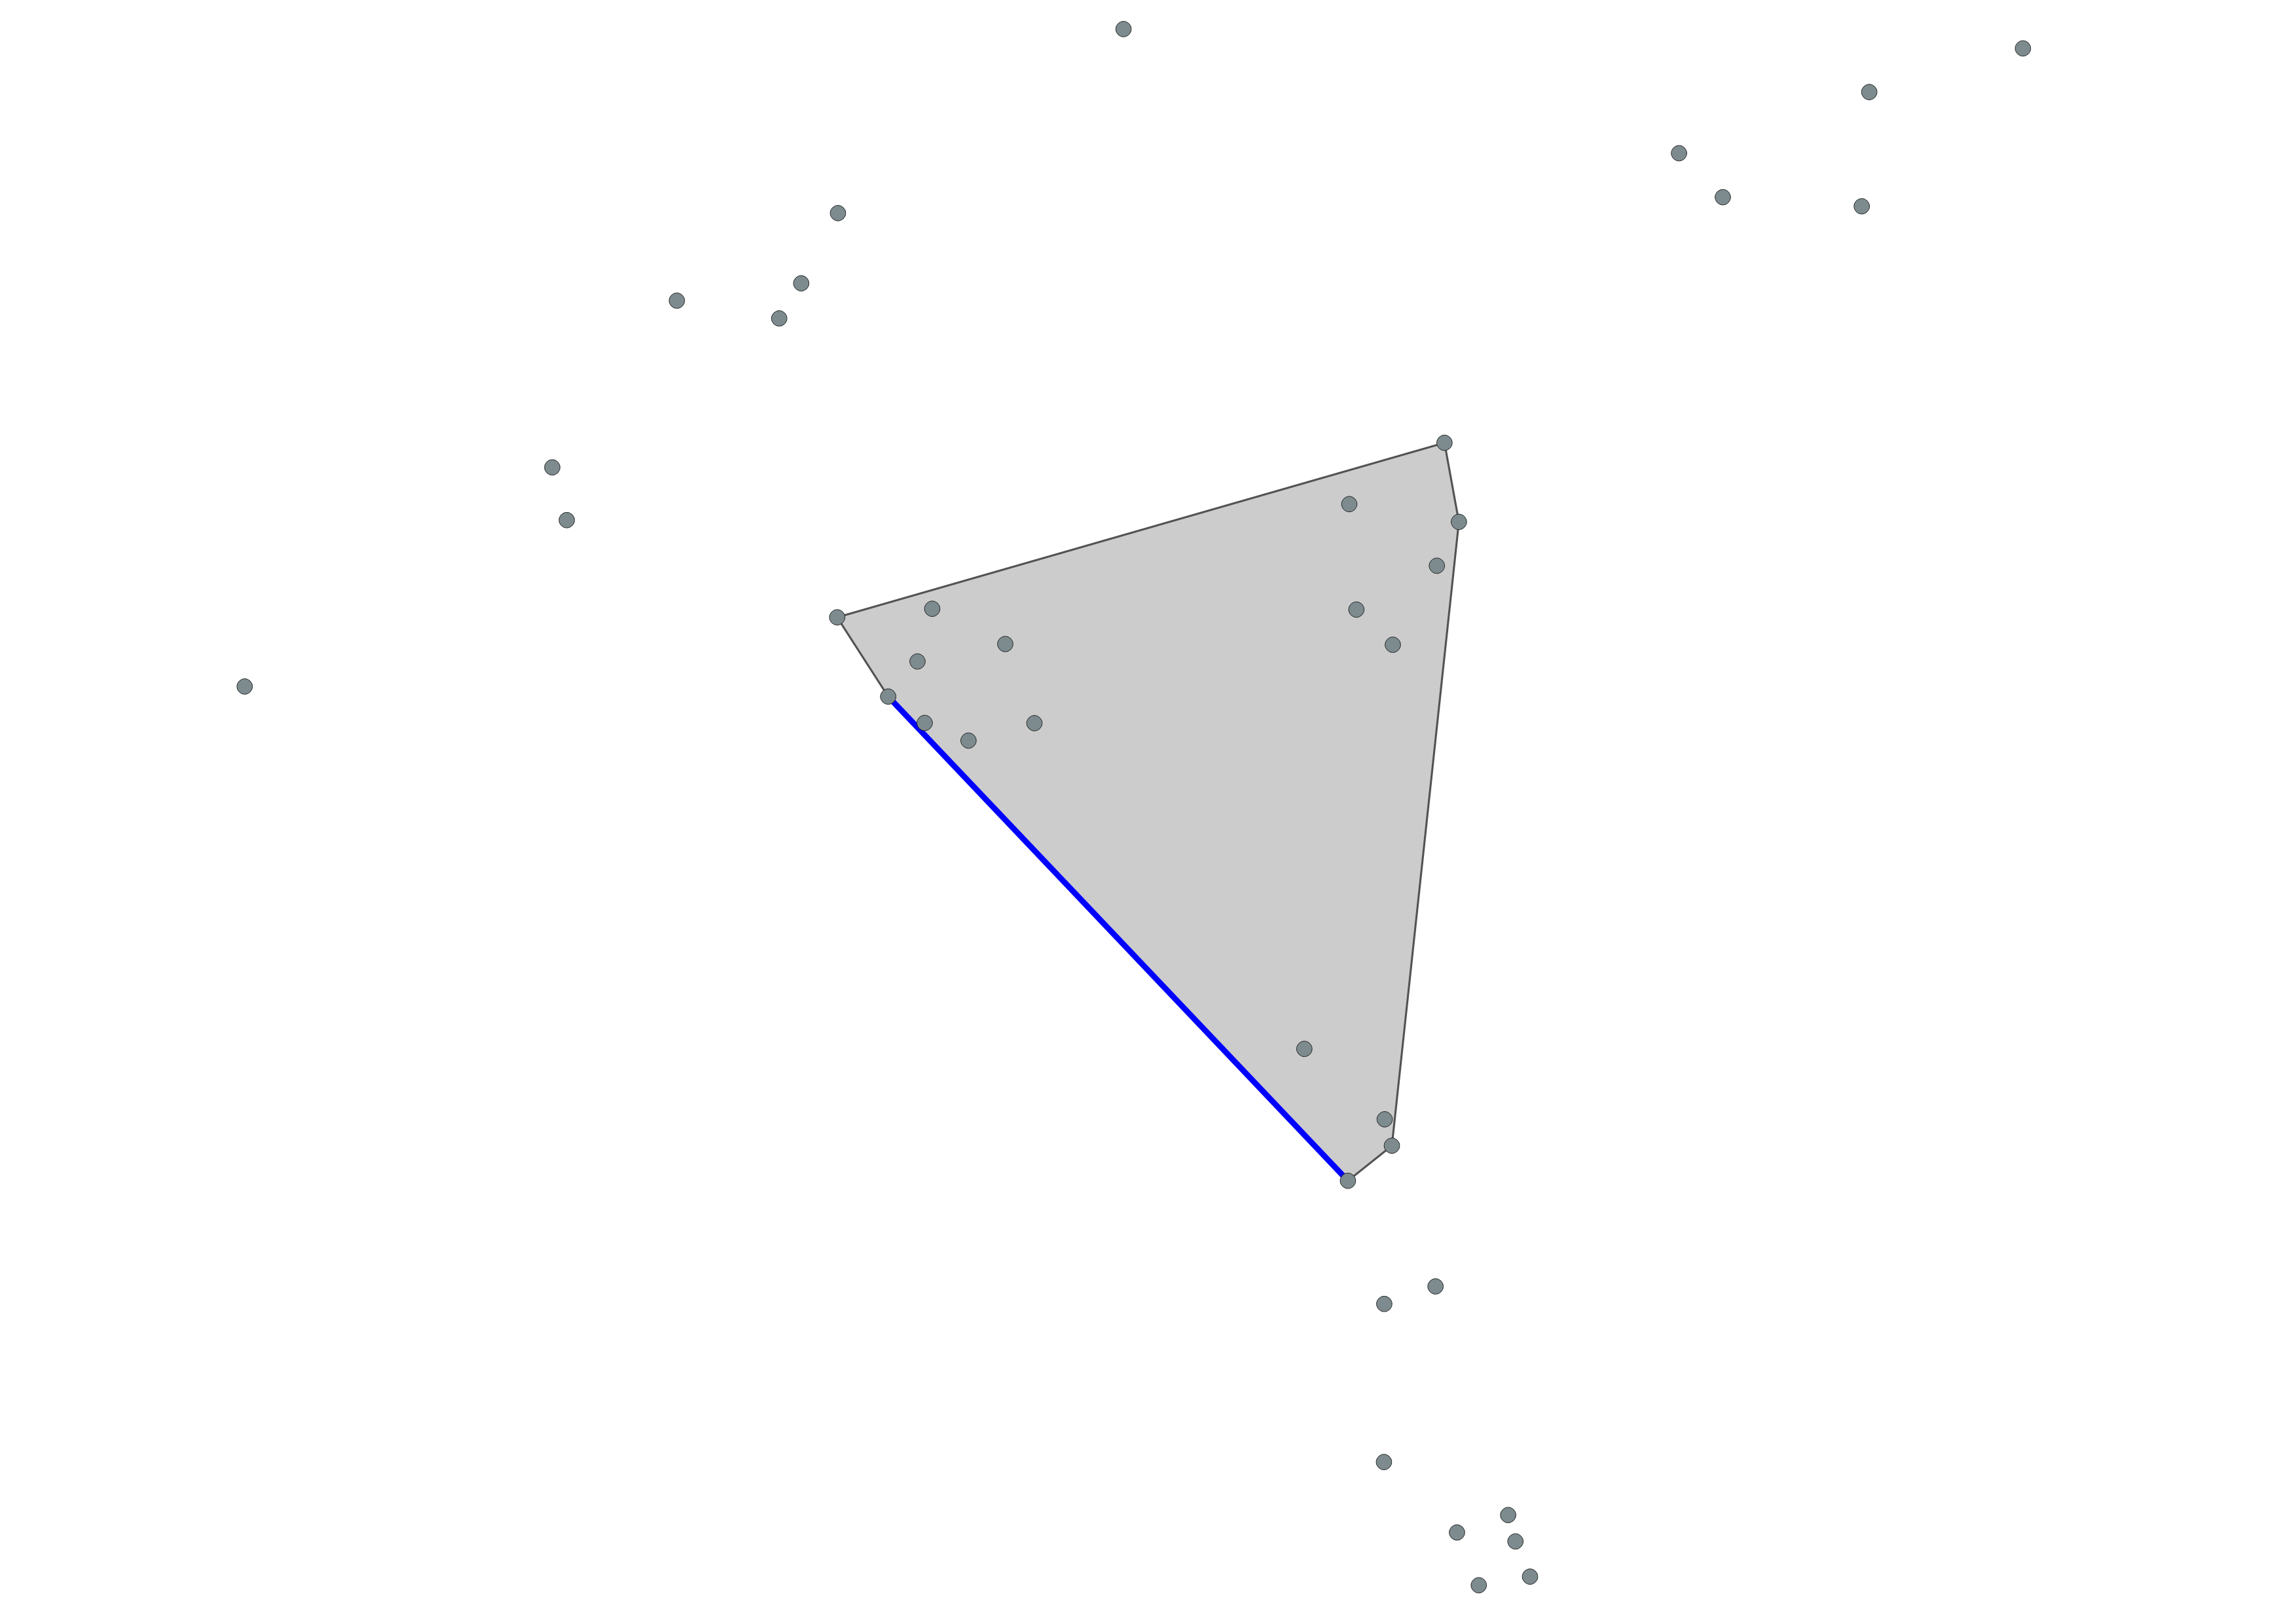
\includegraphics[width=0.85\textwidth]{figures/segment_69}
\end{frame}
\begin{frame}{A first attempt...}{Trace an equilateral triangle of size $\epsilon$}
    \centering
    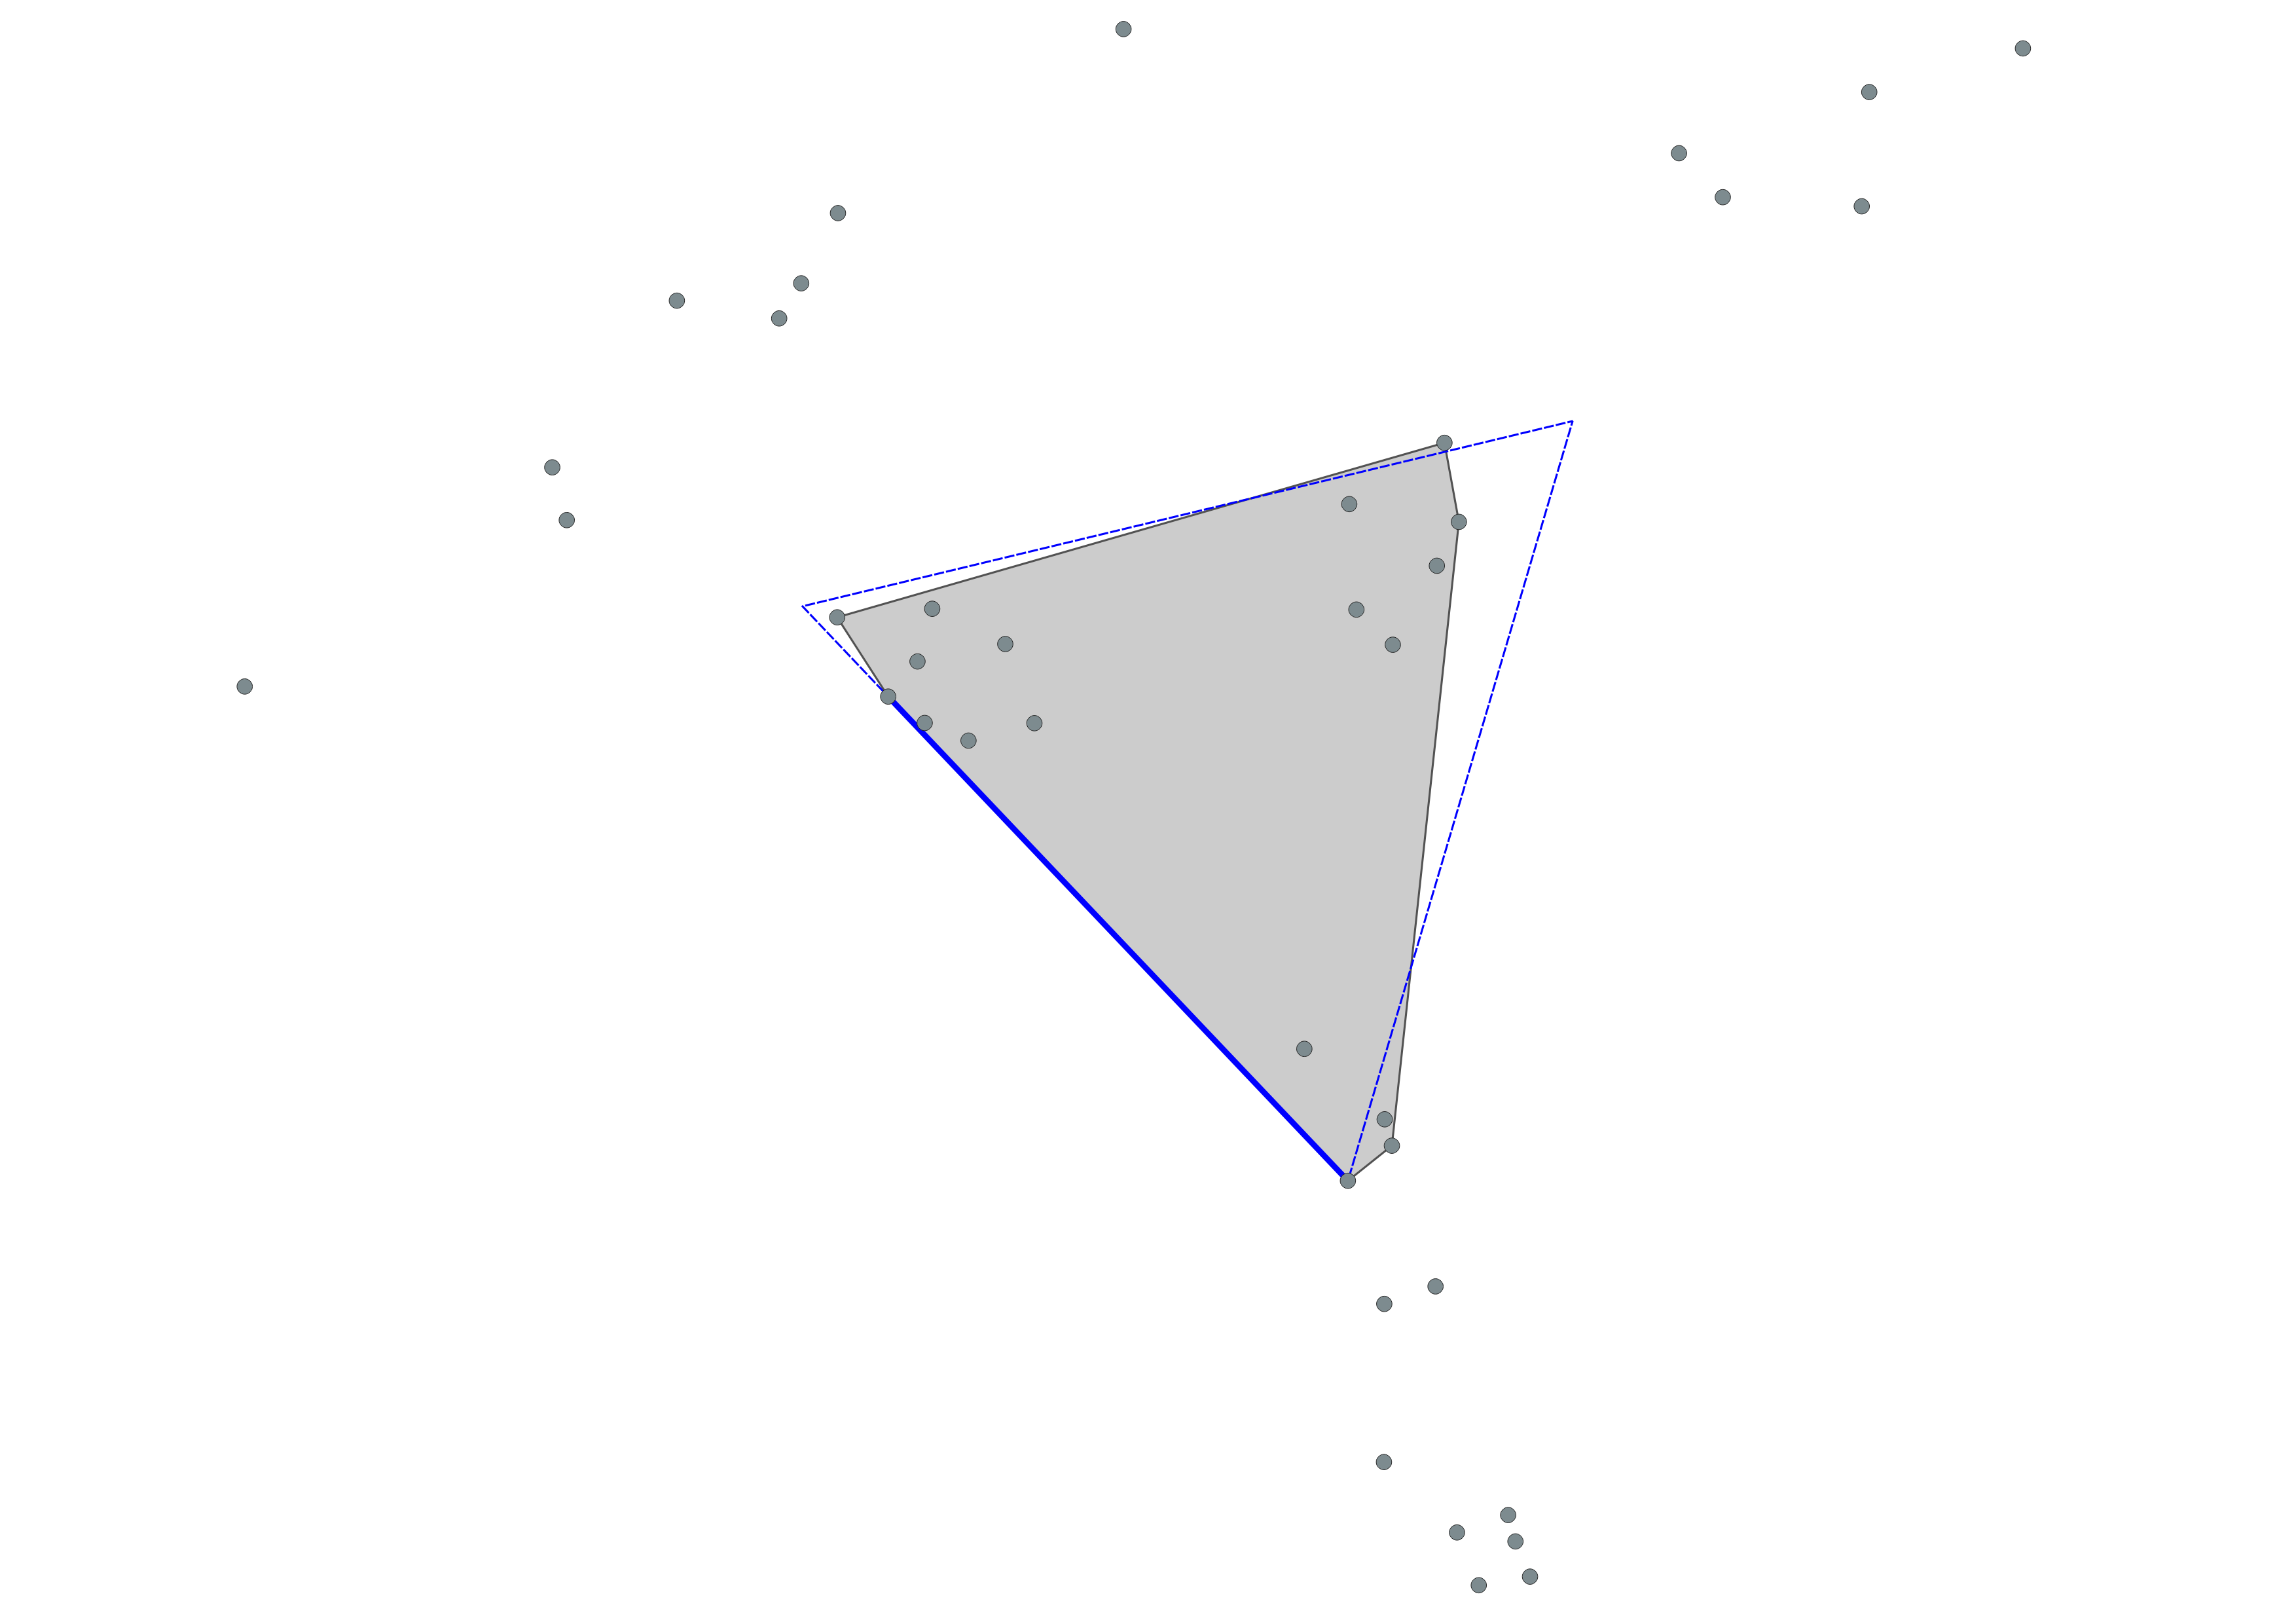
\includegraphics[width=0.85\textwidth]{figures/triangle_69}
\end{frame}
\begin{frame}{A first attempt...}{Locate the centroids of each size}
    \centering
    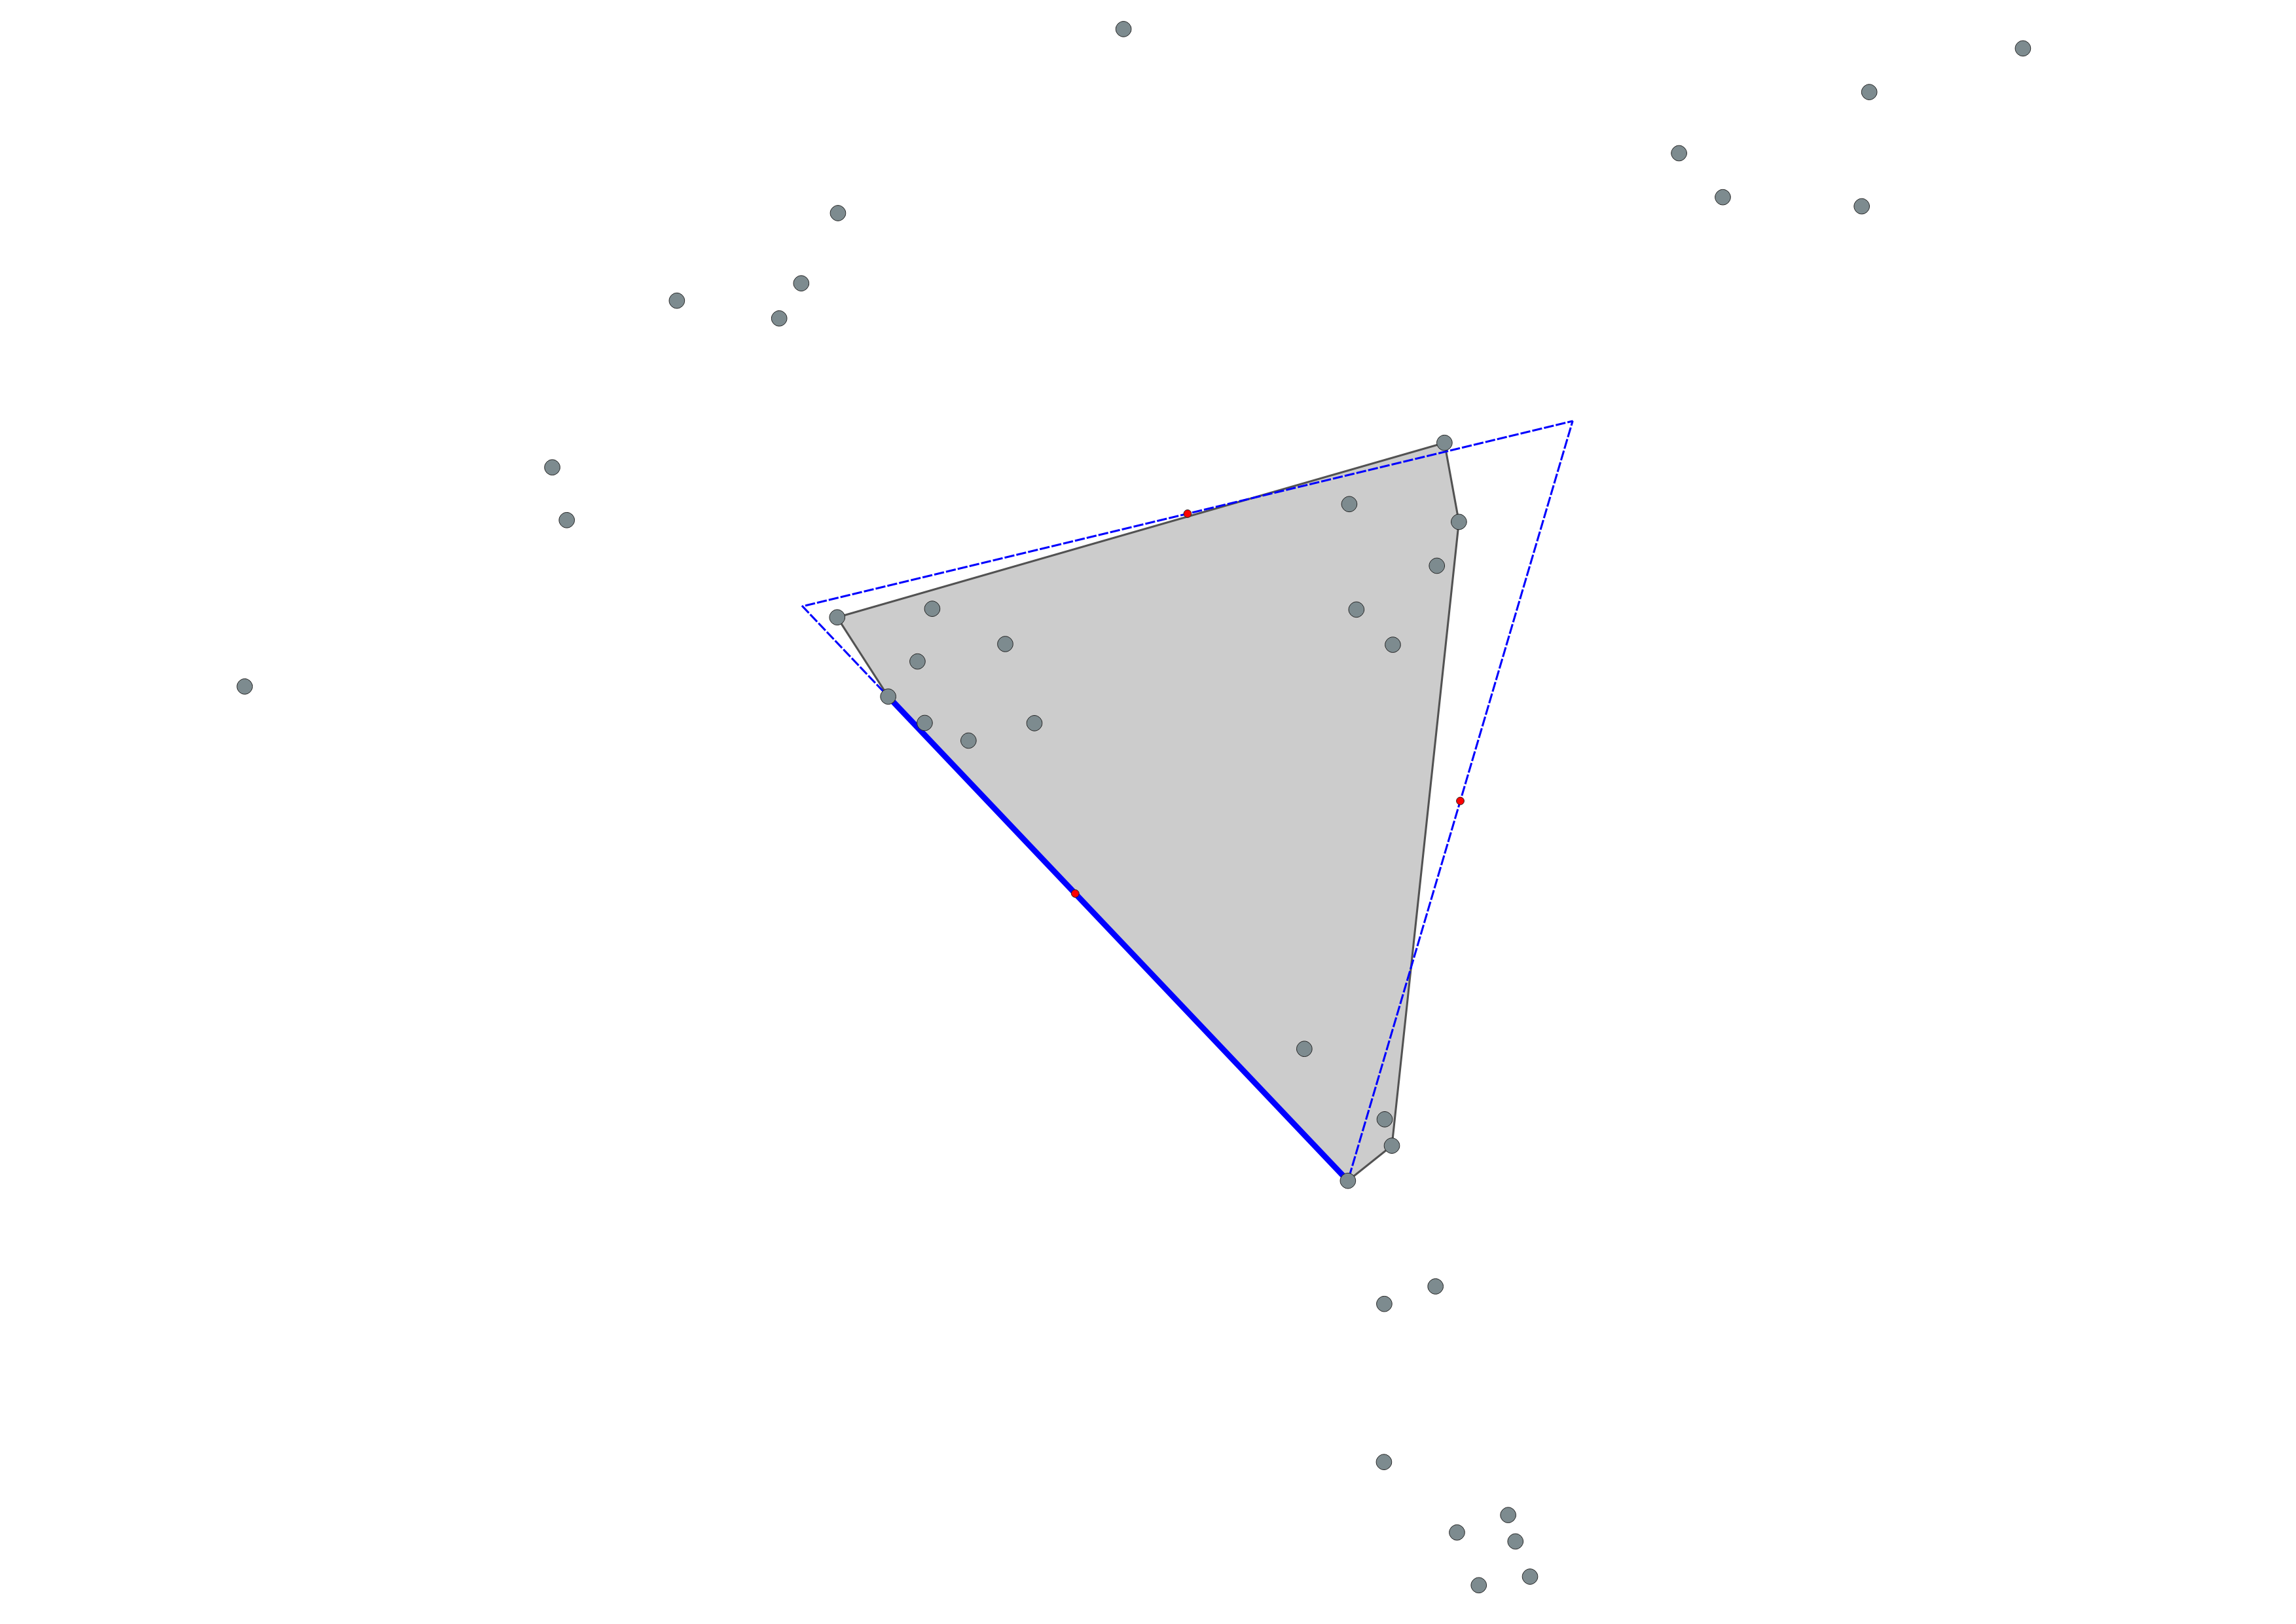
\includegraphics[width=0.85\textwidth]{figures/centroids_69}
\end{frame}
\begin{frame}{A first attempt...}{Draw circles of radius $\epsilon$}
    \centering
    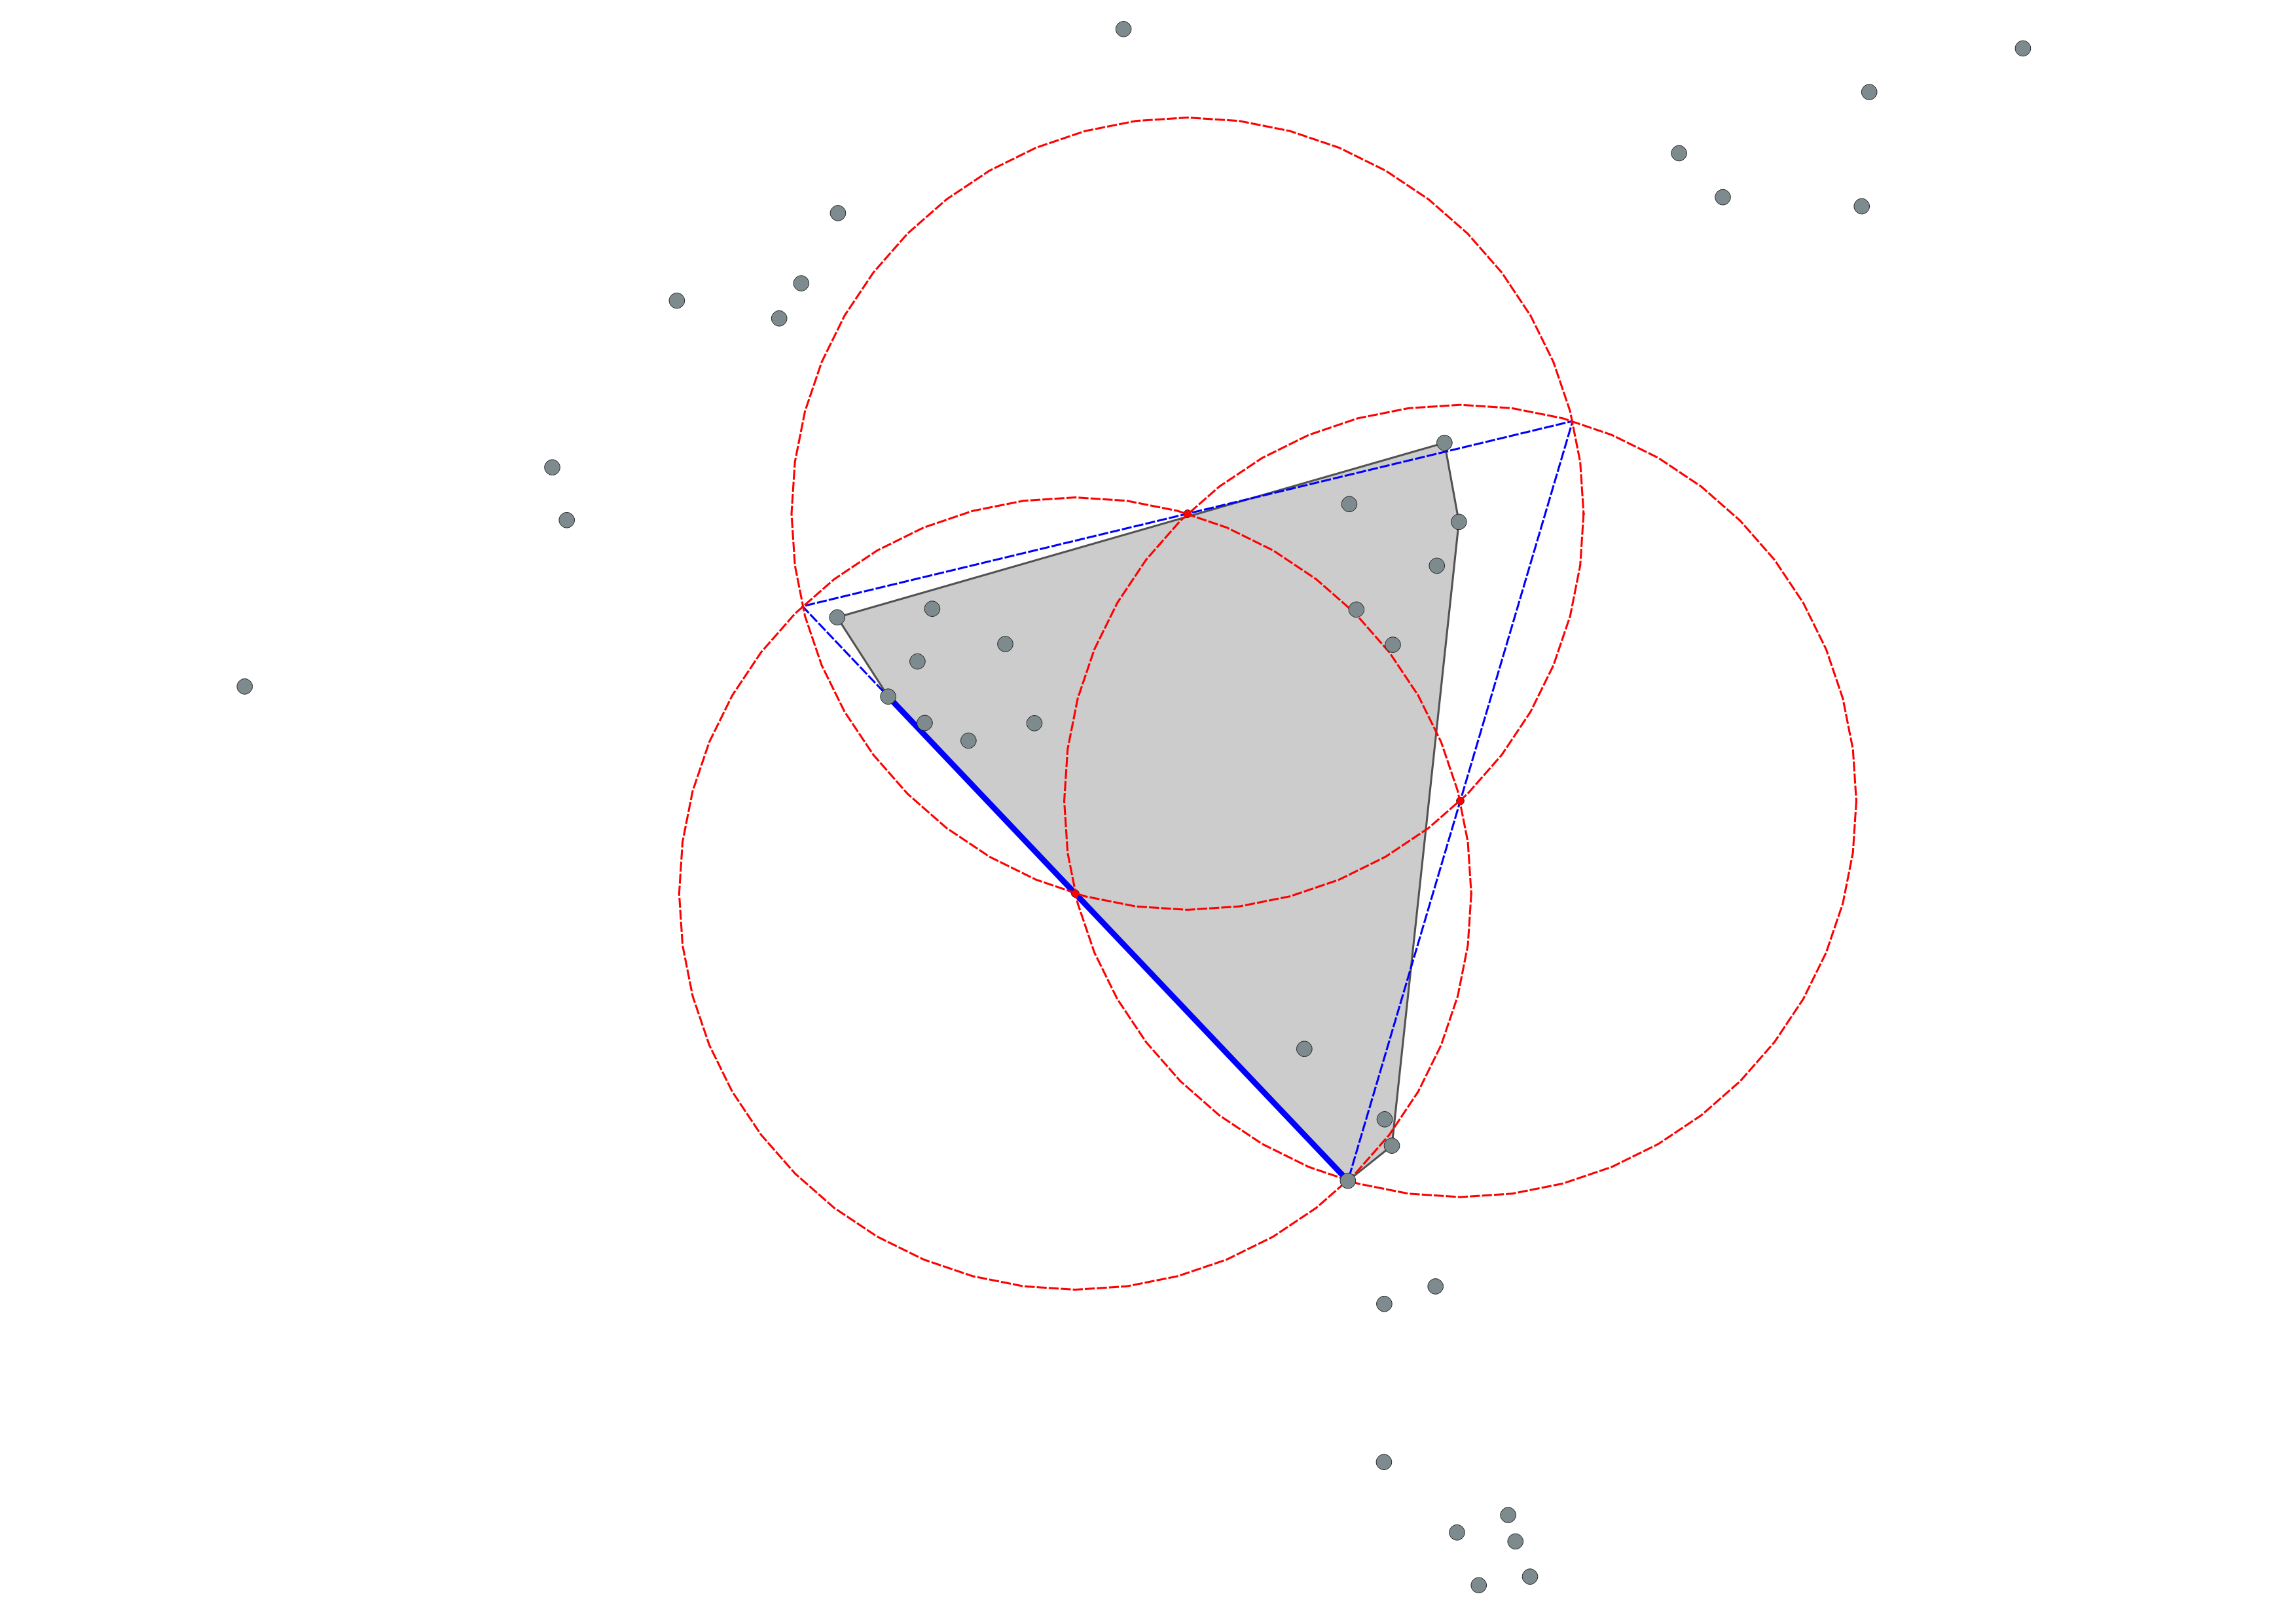
\includegraphics[width=0.85\textwidth]{figures/circles_69}
\end{frame}

\begin{frame}{A first (and wrong) attempt...}{Draw circles of radius $\epsilon$}
    \centering
    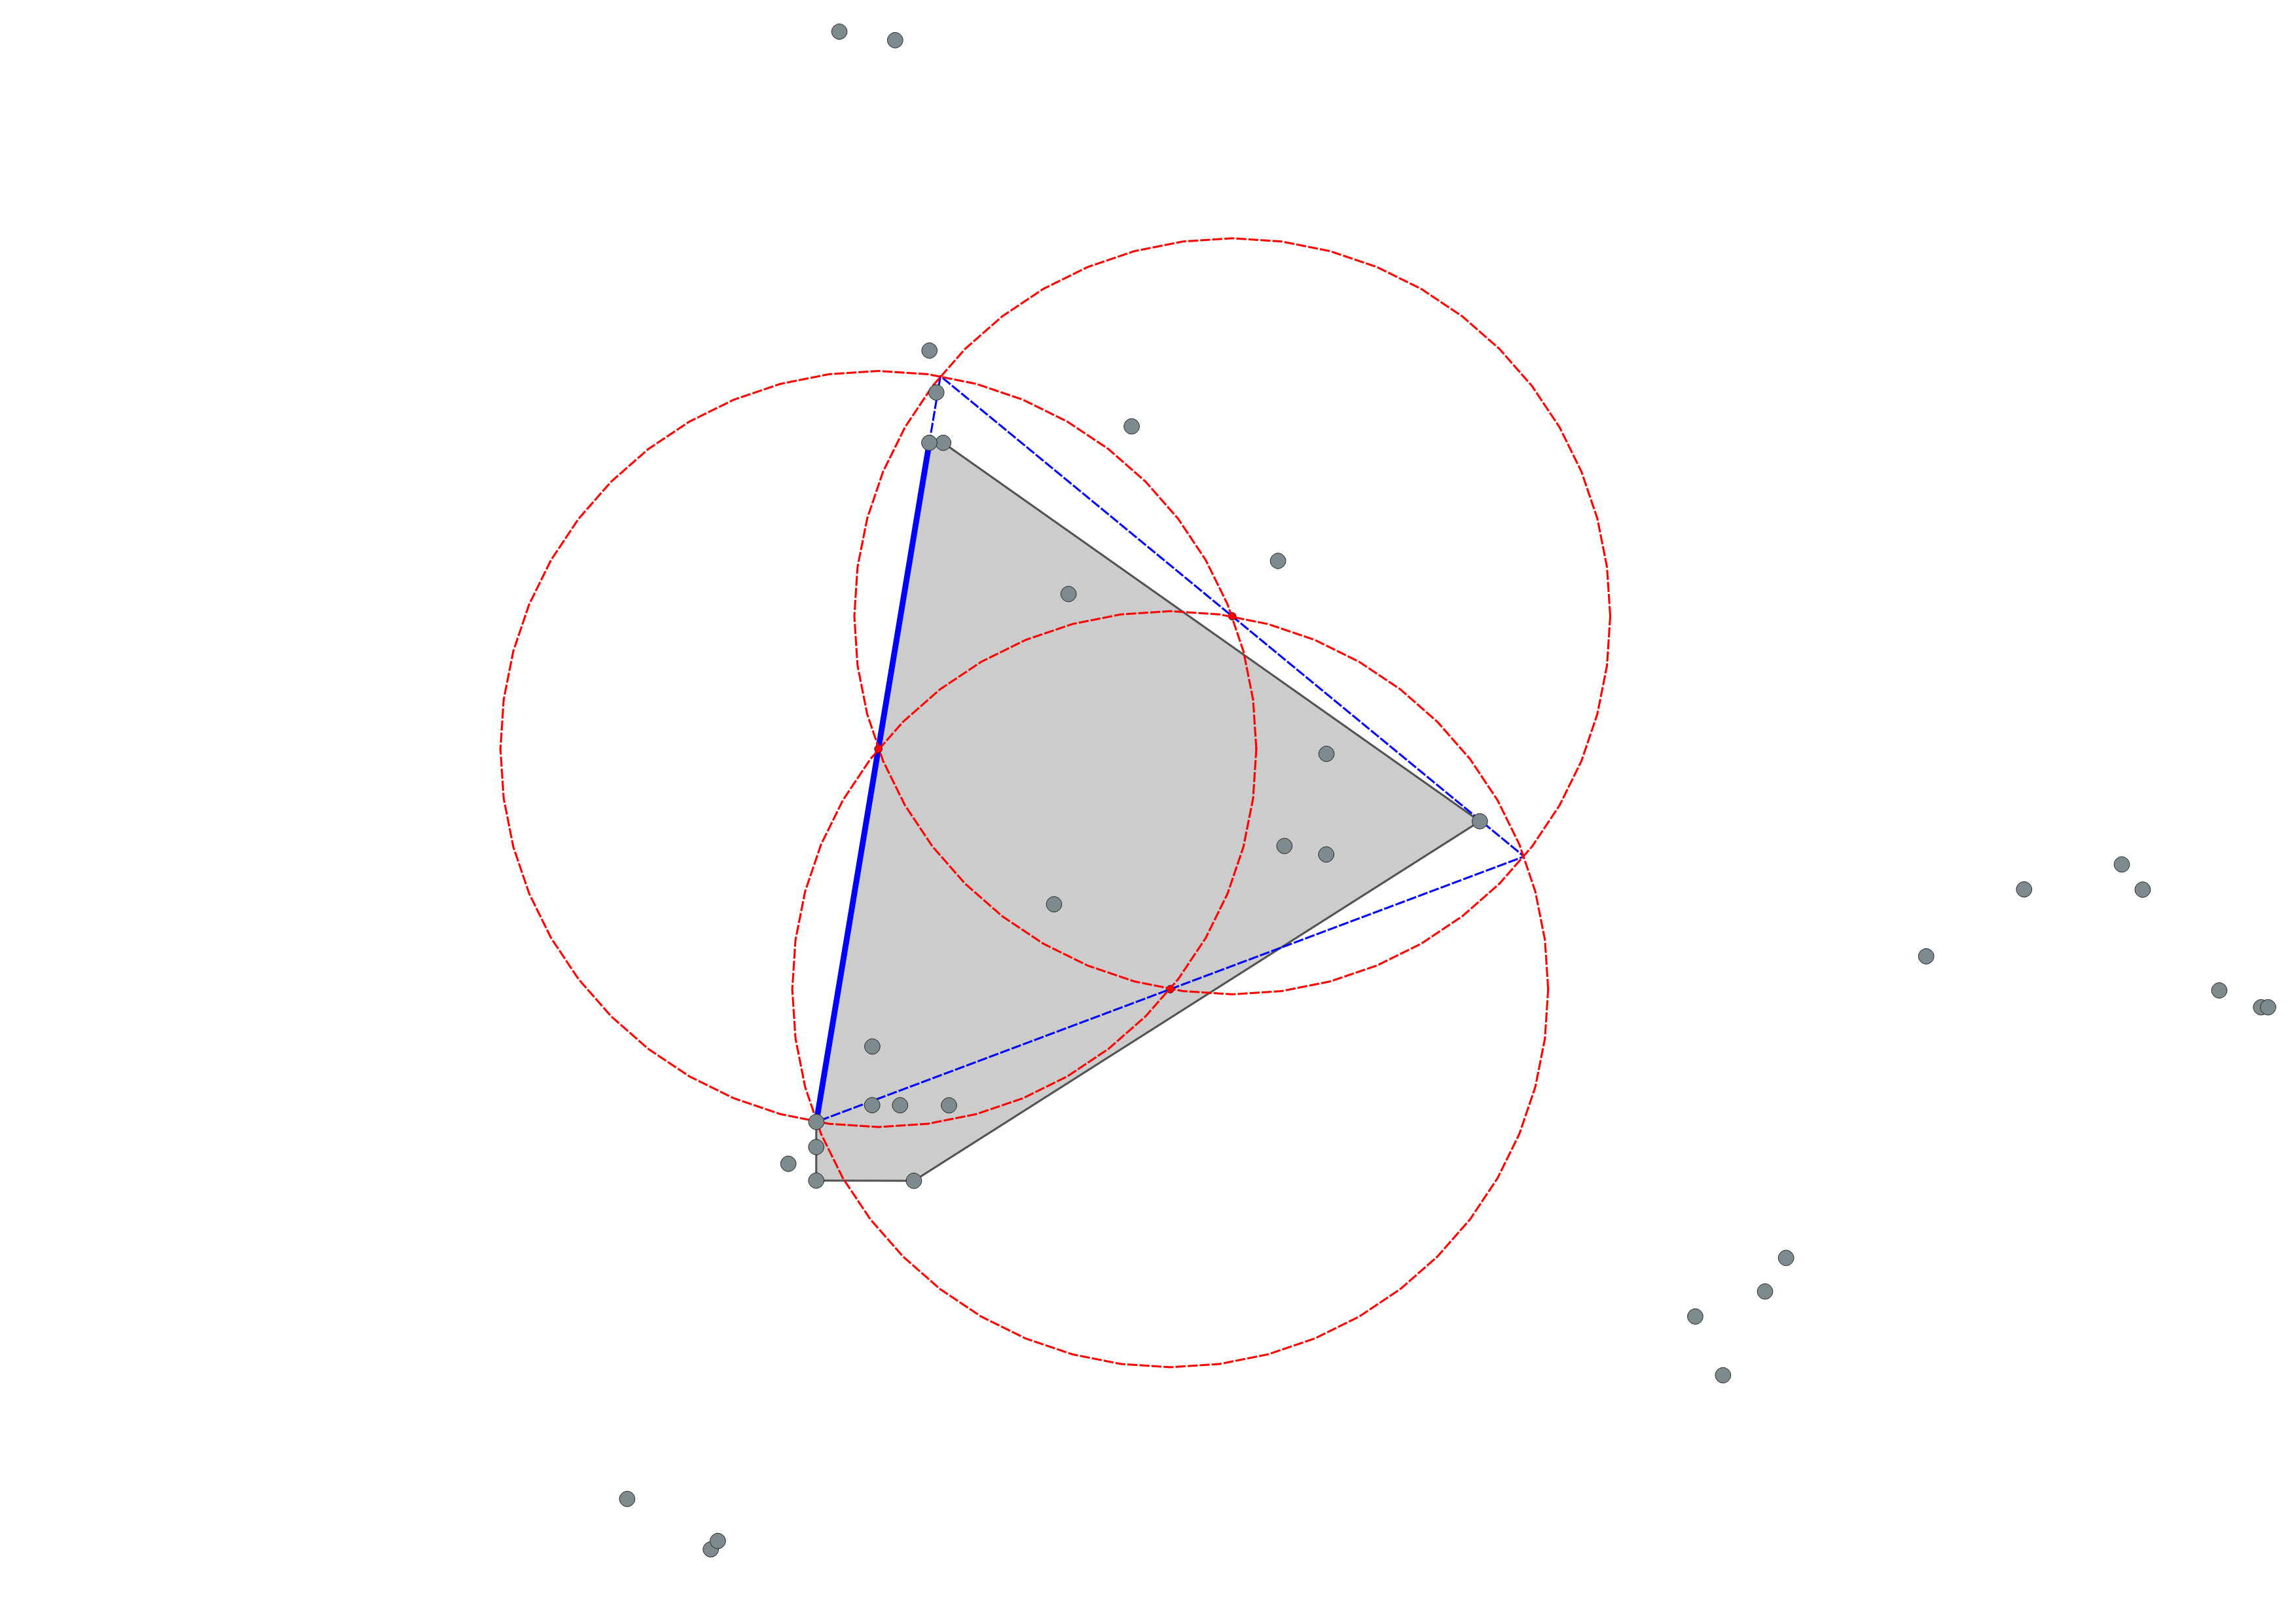
\includegraphics[width=0.85\textwidth]{figures/output_90}
\end{frame}

\begin{frame}{Work in progress...}
    \begin{itemize}
     \item Position: locate the shape's centroid at the MBC's center...
     \item Orientation: align one of the sides of the equilateral triangle parallel to the longest segment in the clique...
    \end{itemize}

    \centering
    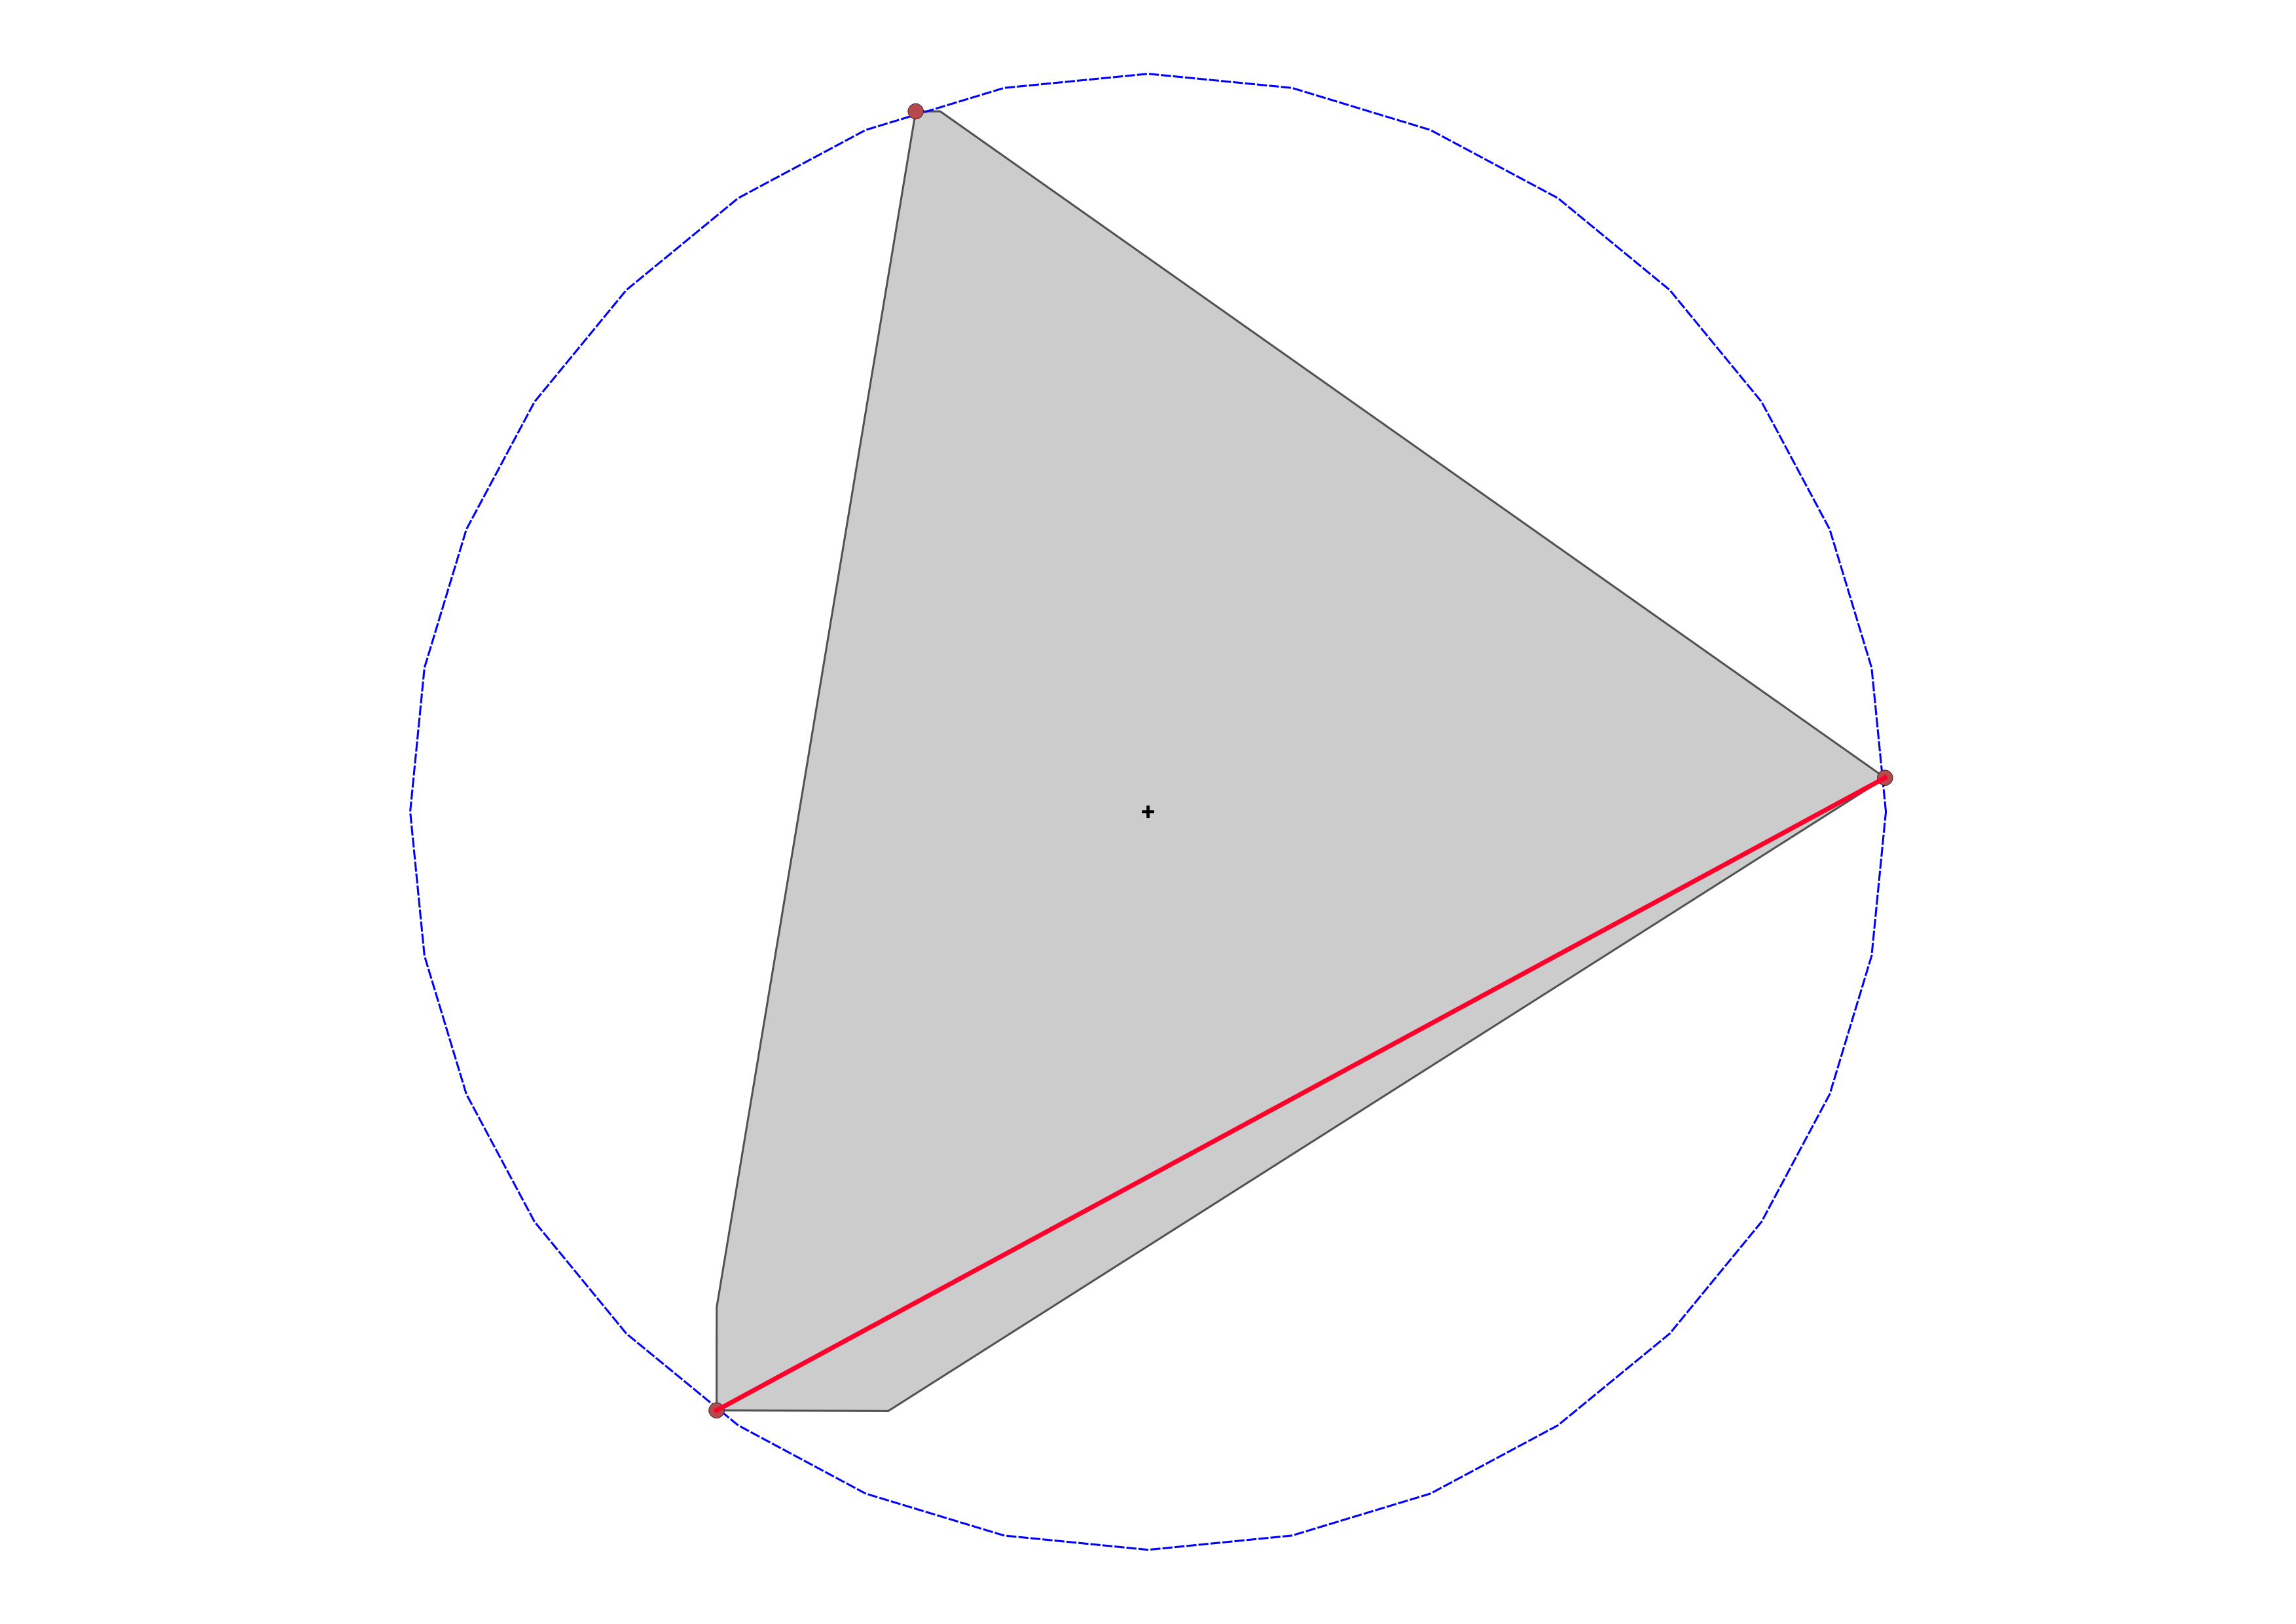
\includegraphics[width=0.65\textwidth]{figures/output2_90}
\end{frame}


\end{document}

